\section{Impedance and offset tuning}

To tune the input impedance of the receiver the input consists of a fixed portion and six resistors which can be switched on, doubled in size between each of them (see section \ref{sec:rx_schematics}). The resulting input impedance values for different codes are shown in figure \ref{fig:rx_imp_tuning_range}. The tuning ranges from \unit[70]{$\Omega$} to \unit[130]{$\Omega$}. Note that this tuning is not linear but as the best code has to be searched for the running link anyway, this leads only to small performance degradation as the tuning is more coarse for higher impedance values as for lower values.

\begin{figure}[H]
  \centering
  {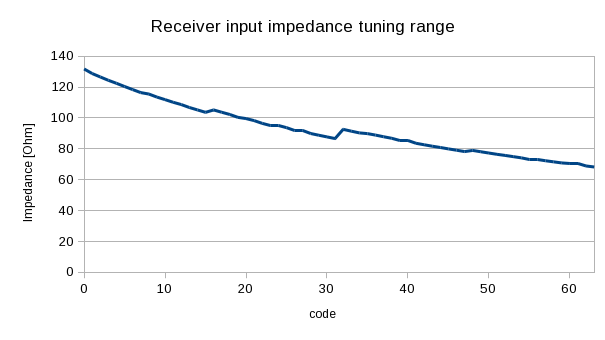
\includegraphics[scale=0.9]{plots/rx_inp_imp.png}}
  \caption{Receiver input impedance tuning range}
  \label{fig:rx_imp_tuning_range}
\end{figure}

The variable offset voltage amplifier enables cancellation of offset voltages (e.g. due to mismatch in the differential pair of the strongARM latch). The achieved offset voltage over input code is shown in figure \ref{fig:voa_offset}. It ranges from \unit[-100]{mV} to \unit[100]{mV} and is pretty much linear. The LSB of the offset tuner gives a tuning of somewhere between 2.55mV and 8.03mV to the offset, these two values are the extremes of the difference in tuning the LSB has.

\begin{figure}[H]
  \centering
  {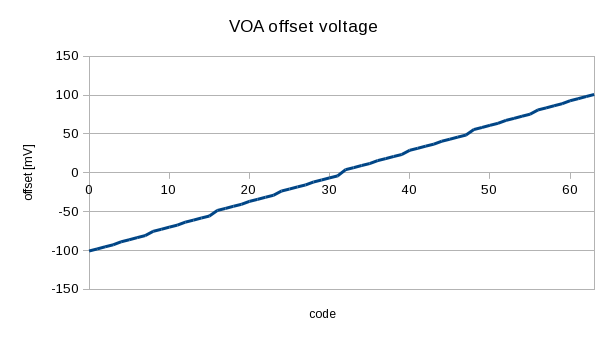
\includegraphics[scale=0.9]{plots/voa_offset.png}}
  \caption{VOA offset voltage tuning range}
  \label{fig:voa_offset}
\end{figure}
